%%%%%%%%%%%%%%%%%%%%%%%%%%%%%%%%%%%%%%%%%%%%%%%%%%%%%%%%%%%%%%%%%%%%%%%%%%%%%%%%
%2345678901234567890123456789012345678901234567890123456789012345678901234567890
%        1         2         3         4         5         6         7         8

\documentclass[letterpaper, 10 pt, conference]{ieeeconf}  % Comment this line out
    % if you need a4paper
%\documentclass[a4paper, 10pt, conference]{ieeeconf}      % Use this line for a4
    % paper

\IEEEoverridecommandlockouts                              % This command is only
    % needed if you want to
    % use the \thanks command
\overrideIEEEmargins
% See the \addtolength command later in the file to balance the column lengths
% on the last page of the document



\usepackage{graphics} % for pdf, bitmapped graphics files
\usepackage{graphicx}
\usepackage{hyperref}
\usepackage{amsmath} % assumes amsmath package installed
\usepackage{amssymb}  % assumes amsmath package installed
\usepackage{subfig}
\usepackage{hyperref}
\usepackage{url}
\usepackage{caption}
\usepackage{refstyle}
\usepackage{times}
\usepackage{epsfig}
\usepackage{graphicx}
\usepackage{amssymb}
\usepackage{algpseudocode}
\usepackage{algorithm}
\usepackage{subfig}
\usepackage{listings}
\usepackage{algpseudocode}
\usepackage{program} 

\title{\LARGE \bf
RRT, Value Iteration and Policy Iteration 
}


\author{Siwei Guo$^{1}$% <-this % stops a space
}


\begin{document}



\maketitle
\thispagestyle{empty}
\pagestyle{empty}

\newcommand{\xn}{x_{near}}
\newcommand{\xr}{x_{rand}}
\newcommand{\xb}{\mathbf{x}}




%%%%%%%%%%%%%%%%%%%%%%%%%%%%%%%%%%%%%%%%%%%%%%%%%%%%%%%%%%%%%%%%%%%%%%%%%%%%%%%%
\section{INTRODUCTION}
Continuous from last week, other than search based path planning algorithm, another major category is sampling based path planning algorithm. Sampling based path planning has a better performance than search based path planning when the dimension of the space is very large. Since for search based path planning, we don't need to keep the whole discretized configuration space, it will be computationally faster and use less memory. In this project, we will mostly focus on RRT. 

We will also discuss (optimal control problem) infinite horizon problems and it's approach. 


\section{Problem Formulation}

\subsection{Static Map and Goal}
Consider the case that there is a map with a known configuration and goal. We would like to find the optimal path that connects the 
start with goal without interfere with any obstacles. The problem is the same as shortest path problem. Given a graph $G$ with 
vertices $x \in \mathcal{X}$, edges and corresponding cost, $C_{ij}$ cost from vertices $x_i$ to node $x_j$. The objective is to find 
the shortest path $Q = \left \{ s, x_1, x_2...,\tau \right \} with \ x_t \in X$ from a start vertices $s$ to an end vertices $\tau$ 
that minimize its corresponding cost is $J^Q =  \sum_{t=1}^{q-1}c_{t,t+1}$. Assume that vertices are not connected to themselves and 
costs are positive values. \\

\textbf{\textit{Problem Formulation}}: 
Find $Q^*$ such that 
\begin{math}
Q = \underset{Q \in \mathbb{Q_{s,\tau}}}{argmin}J^Q
\end{math} with $s\in \mathcal{X}$ and $\tau \in \mathcal{X}$.

\subsection{Optimal Control Problem}
Given a pendulum system with known motion model and cost function, we want to find the optimal control so that we can stabilize the 
inverted pendulum. The state of the system, $\mathbf{x}$ consists of angle of the pendulum, $\theta$, and angular velocity, $\omega$. 
The continuous-time dynamics is $\xb' = d\xb + \xb$. 
Define 
\begin{equation}
d\xb = f(\xb, u) * dt + \sigma * dw
\end{equation}, where $f(\xb, u) = \begin{bmatrix}
\omega \\ 
asin(\theta) - b\omega + u
\end{bmatrix}$, where $a>0$ summarizes the eects of gravity, mass and length of the pendulum, $b > 0$ represents damping and friction, 
u is the control input and $\sigma$ is Gaussian motion noise (Brownian motion). Then define the motion model as
\begin{equation}
    p_f(\cdot \mid \xb_t, \pi_t) =  \mathcal{N}(\xb+f(\xb, u)*dt, \sigma^T\sigma*dt)
\end{equation}

The stage cost is 
\begin{equation}
g(\xb, u) = 1 - exp(kcos(\theta) - k) + \frac{r}{2}u^2
\end{equation}, where $k>0$ determines the shape of the cost and r > 0 scales the control cost. Given these information fo the 
system, we would like to find a policy that minimize the stage cost for each $\xb$.

\textbf{\textit{Problem Formulation}}: 
Given motion model $f(\xb, u)$ and cost function $g(\xb, u)$, find the optimal policy $\pi(\xb)$ such that the cost of policy $\pi$,
$J^{\pi}_0(\xb_0) = \mathbb{E}_{x_{1:T}}\left [  \sum g(\xb_t, \pi_t(\xb_t) \mid \xb_0 \right]$ such that 
$x_{t+1} \sim p_f(\cdot \mid \xb_t, \pi_t)$, $\xb_t \in \mathcal{X}$, $\pi_t(x_t) \in \mathcal{U}(\xb_t)$. 



\section{Technial Approach}
\subsection{Static Map and Goal}
This week, for the motion planning problem, we will use sample based motion planning to solve this problem. The most common 
sampling based motion plan algorithm is RRT. RRT is a tree that constructed from random sampled nodes in the space. The tree
grows until there is a path that connect start and goal. Simple RRT doesn't guarantee to find a path even the number
of nodes goes to infinite. The benefit of RRT is that we don't need to store the whole configuration space and we can find 
a reasonable path in a short amount of computation time even though the path is not optimal. RRT is useful for planning in 
high deminsonal configuration space, such as plan for robot arm, soft robot. 
Start from goal, first randomly sample a point $\xr$ in the space. Find the nearest point in the existing nodes $\xn$.
Then make a connection between $\xr$ and $\xn$ and extend $\xn$ a small distance, $\sigma$, towards $\xr$ if there is no obstacles.
If there are obstacles in the middle, we pick the point that is at the edge of the obstacles to be $\xn$.
Repeat this step until the goal is connected. 
To ensure that the goal can be sampled, for every 100 iteration, set $x_{goal}$ as $\xr$. If there exist a path between goal and 
one of the node which is collision free, we can include the goal to the tree and stop planning. \\

I have also add a heuristic to the sampling process. Instead of sampling from a uniform distribution, $\xr$ is sampled through 
a gaussian distribution which the mean is the goal, $\sim \mathcal{N}(x_{goal}, \sigma)$. $\sigma$ determines how spread 
$\xr$ should be. For the case that there is not many obstacles, adding a heuristic can help find a path in less iterations. However, 
for the case that there is many obstacles in the map, adding heuristic might cause robot to stuck at a corner. 

\begin{algorithm}[H]
\caption{RRT}\label{alg:RRT1}
\begin{algorithmic}[1]
\State{$\tau$.init($x_s$)}
\For{$i = 1 ... N$}
\State{Sample $x_{rand}$}
\State{Extend($\tau$, $x_rand$)}
\EndFor
\end{algorithmic}
\end{algorithm}

\begin{algorithm}[H]
\caption{Extend($\tau$, $x_rand$)}\label{alg:RRTe}
\begin{algorithmic}[1]
\State{$x_{near} \leftarrow$ NearestNeighbor($\tau$, $x_{rand}$)}
\State{$x_{new} \leftarrow$ Steer($x_{near}, x_{rand}$)}
\If{ObsacleFree($x_{near}, x_{rand}$), then}
\State{$\tau$.add vertex($x_{new}$)}
\State{$\tau$.add edge($x_{new}$, $x_{near}$)}
\If{$x_{new} = x_{rand}$}
\Return{Reached}
\EndIf
\EndIf
\end{algorithmic}
\end{algorithm}


\subsection{Optimal Control}
First, we will discretize the state space and control space. The pendulum degree is in the range of 
$\left [ -\pi, \pi \right ]$ and we split into $n_1$ grids, same for control $u \in \left [ -u_{min}, u_{max} \right ]$ with 
discretization of $n_u$ grids and angular velocity $\omega \in \left [ -u_{min}, u_{max} \right ]$ with discretization of 
$n_2$. Becasue the motion model contains Gaussian motion noise and discretization, for $\xb'$ we will pick the points that 
is within one standard deviation of $\mathcal{N}(\bar{\xb}, \sigma^T\sigma*dt)$. For this setup, we need to solve a
inifinite-horizon problem. As terminal time $T$ goes to infinity, the original problem, 
$min \ J^{\pi}_0(\xb_0) = \mathbb{E}_{x_{1:T}}\left [  \sum g(\xb_t, \pi_t(\xb_t) \mid \xb_0 \right]$ becomes a time 
invariant cost-to-go problem. Since there is no terminal state, but future reward should weighted less
than current rewards. Then we can formulate a dicounted infinite horizon problem which is stationary, 
\begin{equation}
    \begin{aligned}
    J^*(x) =
        & \underset{u\in \mathcal{U}}{\text{min}}
        & & g(\xb, u) + \gamma \mathbb{E}_{x'\sim p_f(\cdot \mid \xb, u)} \left [ J^*(\xb') \right ] \text{,} \ \forall \xb \in \mathcal{X} \\
    \end{aligned}
\end{equation}
This is also the Bellman Equation
\begin{equation}
    \begin{aligned}
    J^*(i) =
        & \underset{u\in \mathcal{U}}{\text{min}}
        & & g(i, u) + \gamma \sum \left [ P_{ij}^u J^*(j) \right ] \text{,} \ \forall i \in \mathcal{X} \\
    \end{aligned}
\end{equation}
This could be solved using policy iteration or value iteration if the policy statisfies follow two assumptions
\begin{itemize}
    \item Proper Stationary Policy: a policy $\pi$ for which there exists int(m) that $P(x_m = 0 \mid x_0 = i) > 0 \forall i \in
    \mathcal{X}$ 
    \item Proper Policy Assumption: there should exists at least one proper policy $\pi$
  \end{itemize}  


\section{CONCLUSIONS}
\subsection{Static Map and Goal}
With RRT and enough time, we are able to find a path for both map. For triangle map, compare to the optimal path, RRT algorithm
isn't able to sample points in a very narrow space. The optimal path requires to go through a very narrow corridor. For RRT, it is 
nearly impossible. Therefore, it didn't find the optimal path. However, RRT finds a suboptimal path with only 2246
sampled points. Since we add a heuristic to the sampling process, more points were sampled at upper right corner which causes the
path to go up first instead of go though the bottom which seems to be a better path. \\

For maze map, the algorithm sampled 121852 points before finding the path which tooks about 4hs. At first, the heuristic for sampling
is relatively large. It took even larger amount of points to find a path. Since in the maze case, we don't want the algorithm to be 
greedy. Instead, we want it find the small exit on each wall. However, even after I remove the heuristic, it still takes a long time
to find a path. From fig3 we can see that, sampled points have alomst take over all the space inside the second outermost wall.
I also didn't let goal to be $\xr$ in every 100 steps to save time. As long as the robot can escape the maz, the path for 
the last distance from the exit of maze to the goal can be easily found using heuristic. I chose $\epsilon$ to be 0.5. For 
larger $\epsilon$, it took less time to find the path. However, $\epsilon$ cannot be too large, otherwise the $\xn$ will frequently 
collide with obstacles. 

\begin{figure}[h]
    \centering
    \subfloat[Triangle]{{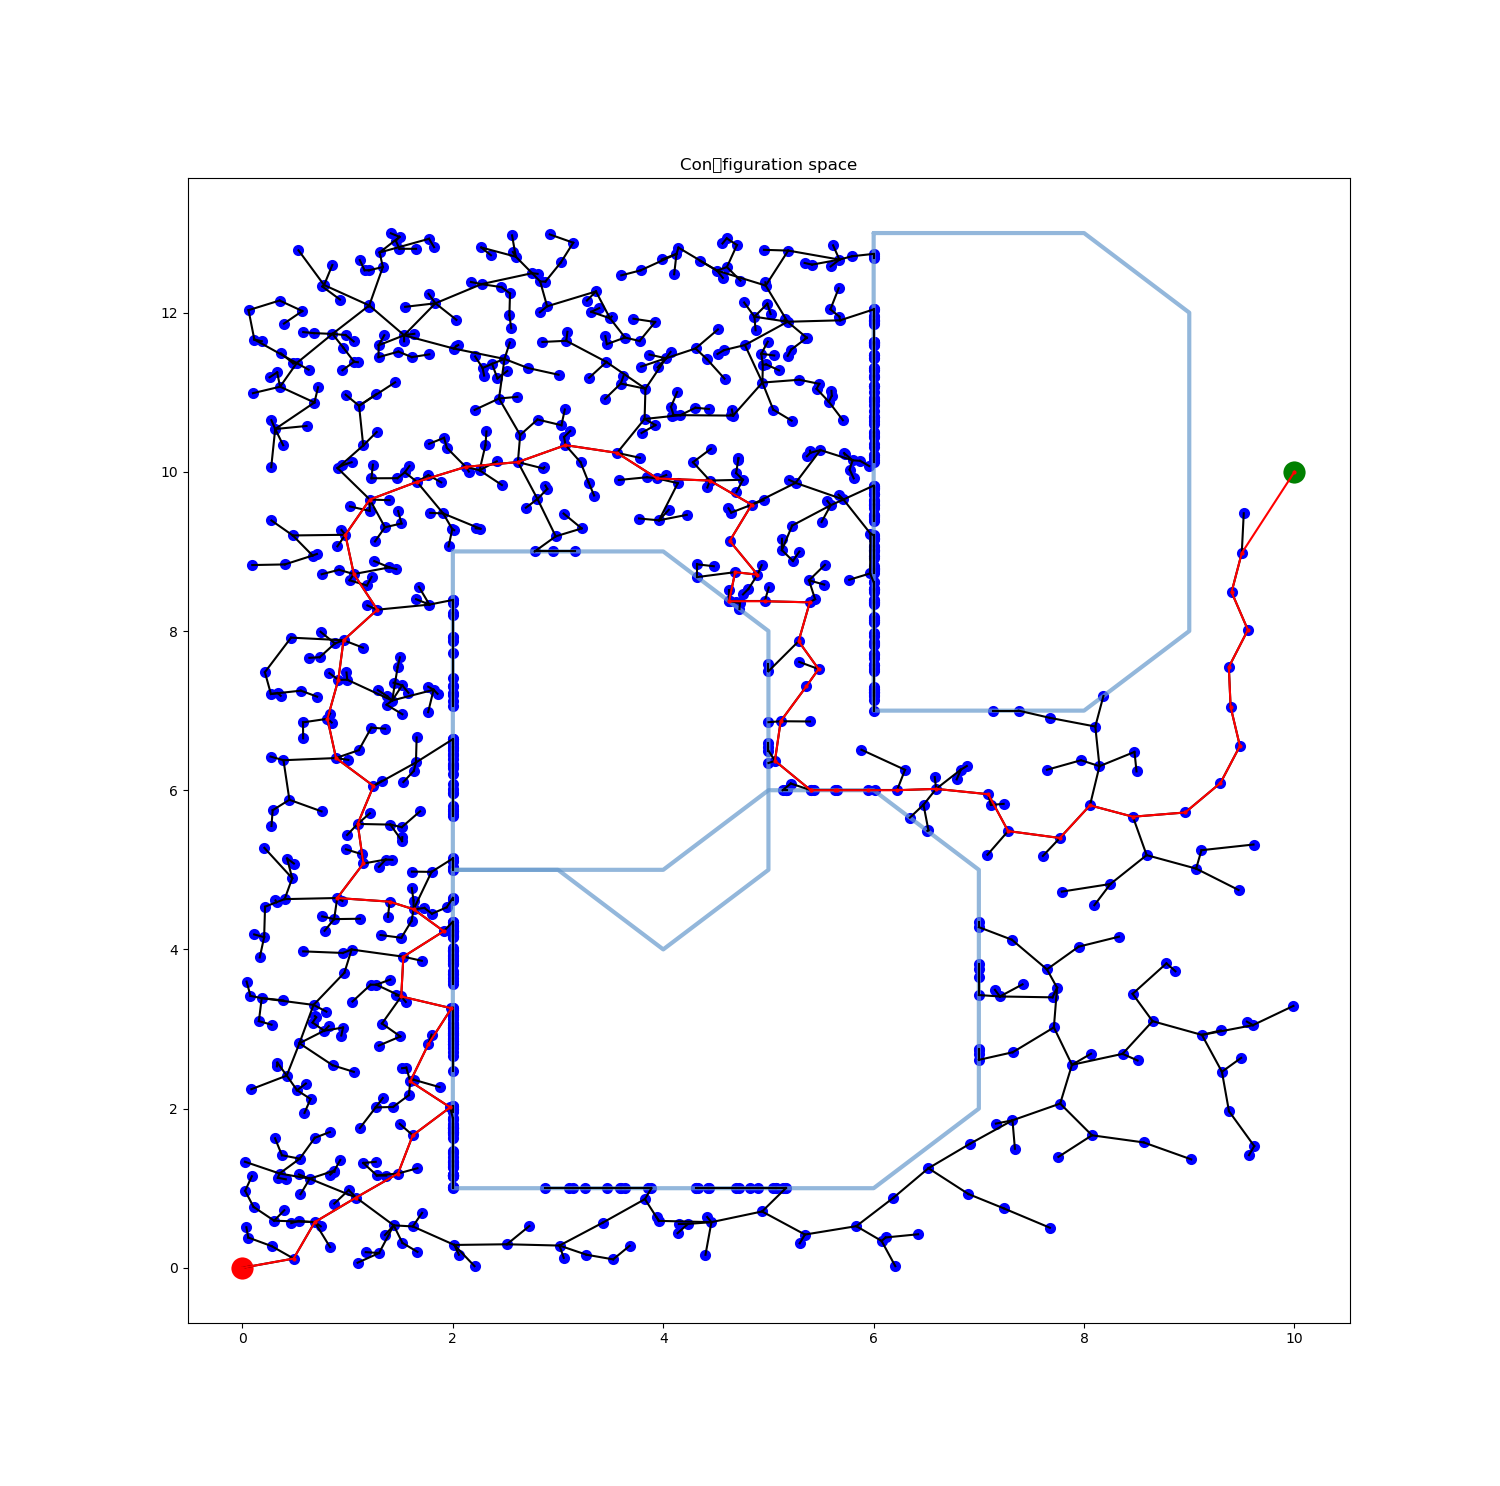
\includegraphics[width=6cm]{tri_2246_66.png} }}
    \caption{RRT: Trangle Map. 2246 sampled points. 66 nodes from start to goal}
    \label{fig:map1}
 \end{figure}

 \begin{figure}[h]
    \centering
    \subfloat[Triangle]{{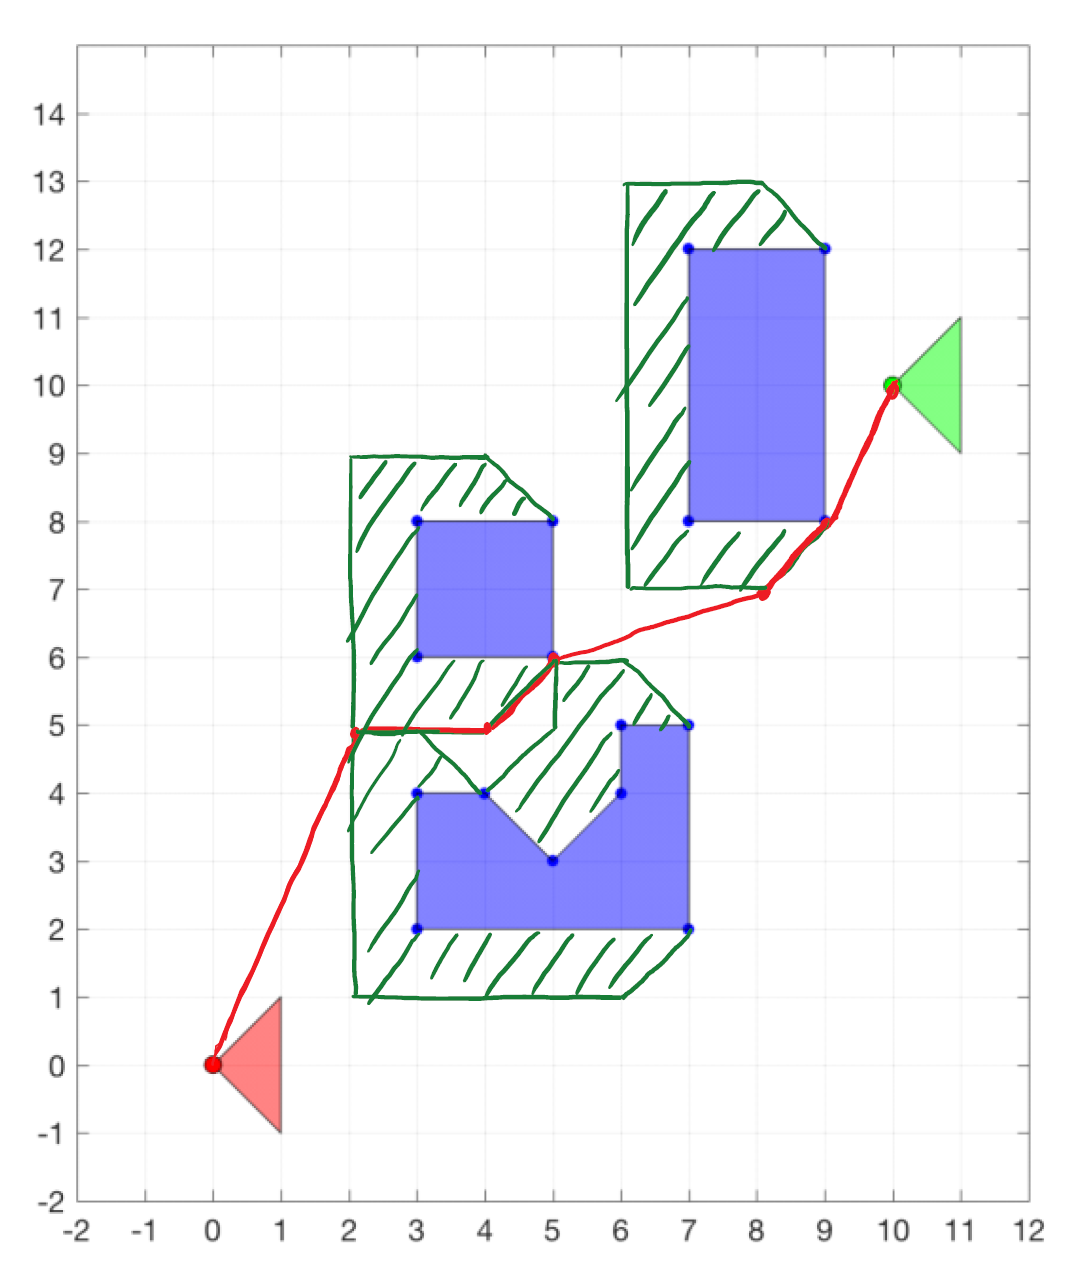
\includegraphics[width=6cm]{org.png} }}
    \caption{Trangle Map. Optimal Path}
    \label{fig:map1}
 \end{figure}

 \begin{figure}[h]
    \centering
    \subfloat[Triangle]{{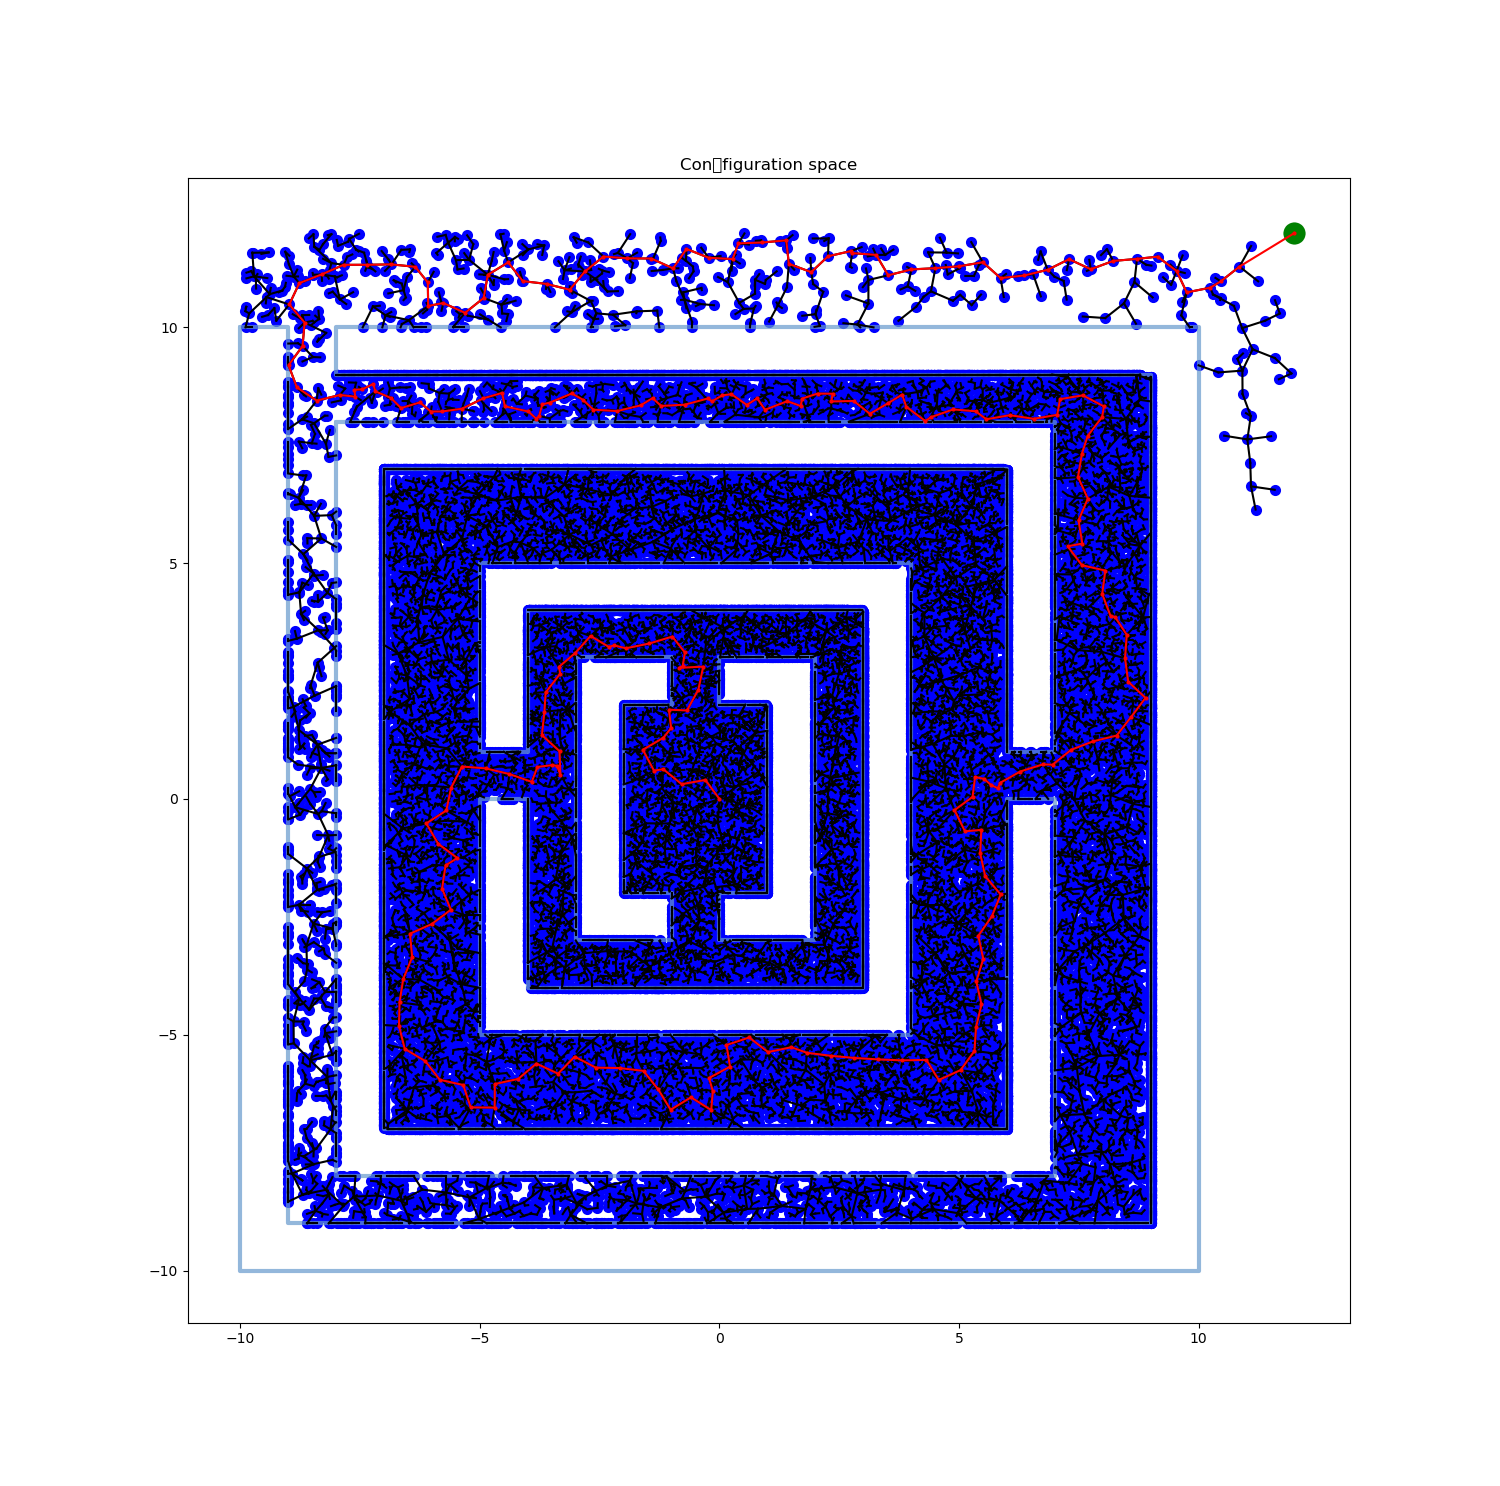
\includegraphics[width=6cm]{maz_121852_240.png} }}
    \caption{RRT: Maze Map. 121852 sampled points. 240 nodes from start to goal}
    \label{fig:map1}
 \end{figure}

 \subsection{Optimal Control}
 



% \addtolength{\textheight}{-12cm}   % This command serves to balance the column lengths
% on the last page of the document manually. It shortens
% the textheight of the last page by a suitable amount.
% This command does not take effect until the next page
% so it should come on the page before the last. Make
% sure that you do not shorten the textheight too much.

%%%%%%%%%%%%%%%%%%%%%%%%%%%%%%%%%%%%%%%%%%%%%%%%%%%%%%%%%%%%%%%%%%%%%%%%%%%%%%%%



%%%%%%%%%%%%%%%%%%%%%%%%%%%%%%%%%%%%%%%%%%%%%%%%%%%%%%%%%%%%%%%%%%%%%%%%%%%%%%%%





\end{document}